% cSpell:ignore DBLP manuallabel

\begin{frame}{Max stash size grows linearly with $\lambda$}
	
	\begin{center}

		\begin{figure}\manuallabel{fig:max-stash-size-linear}{figure}
				
			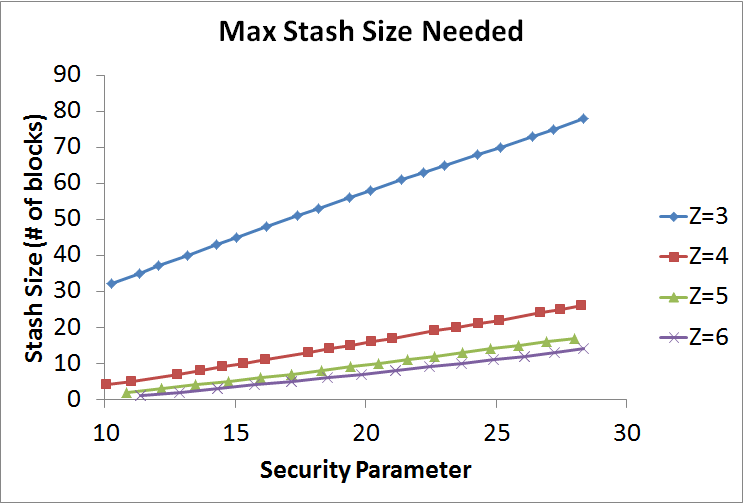
\includegraphics[
				height=5cm,
				keepaspectratio
			]{static/images/max-stash-size-linear.png}
				
		\end{figure}
		
	\end{center}

	Figure 3 from~\cite{DBLP:journals/corr/abs-1202-5150}.

\end{frame}

\begin{frame}{Max stash size for large security parameters}
	
	\begin{center}

		\begin{figure}\manuallabel{tbl:stash-size-for-sec-parameters}{table}

			\begin{tabular}{ l c c c }

				\toprule%

				\multirow{3}{*}{\textbf{Security parameter} $\lambda$}	& \multicolumn{3}{c}{\textbf{Bucket size} $Z$}					\\
																		& 4												& 5		& 6		\\
																		& \multicolumn{3}{c}{\textbf{Max stash size}}					\\

				\midrule%

				80														& 89											& 63	& 53	\\
				128														& 147											& 105	& 89	\\
				256														& 303											& 218	& 186	\\

				\bottomrule%

			\end{tabular}

		\end{figure}

	\end{center}

	Figure 5 from~\cite{DBLP:journals/corr/abs-1202-5150}.

\end{frame}

\begin{frame}{Max stash size does not depend on $N$}
	
	\begin{center}

		\begin{figure}\manuallabel{fig:stash-size-does-not-depend-on-n}{figure}

			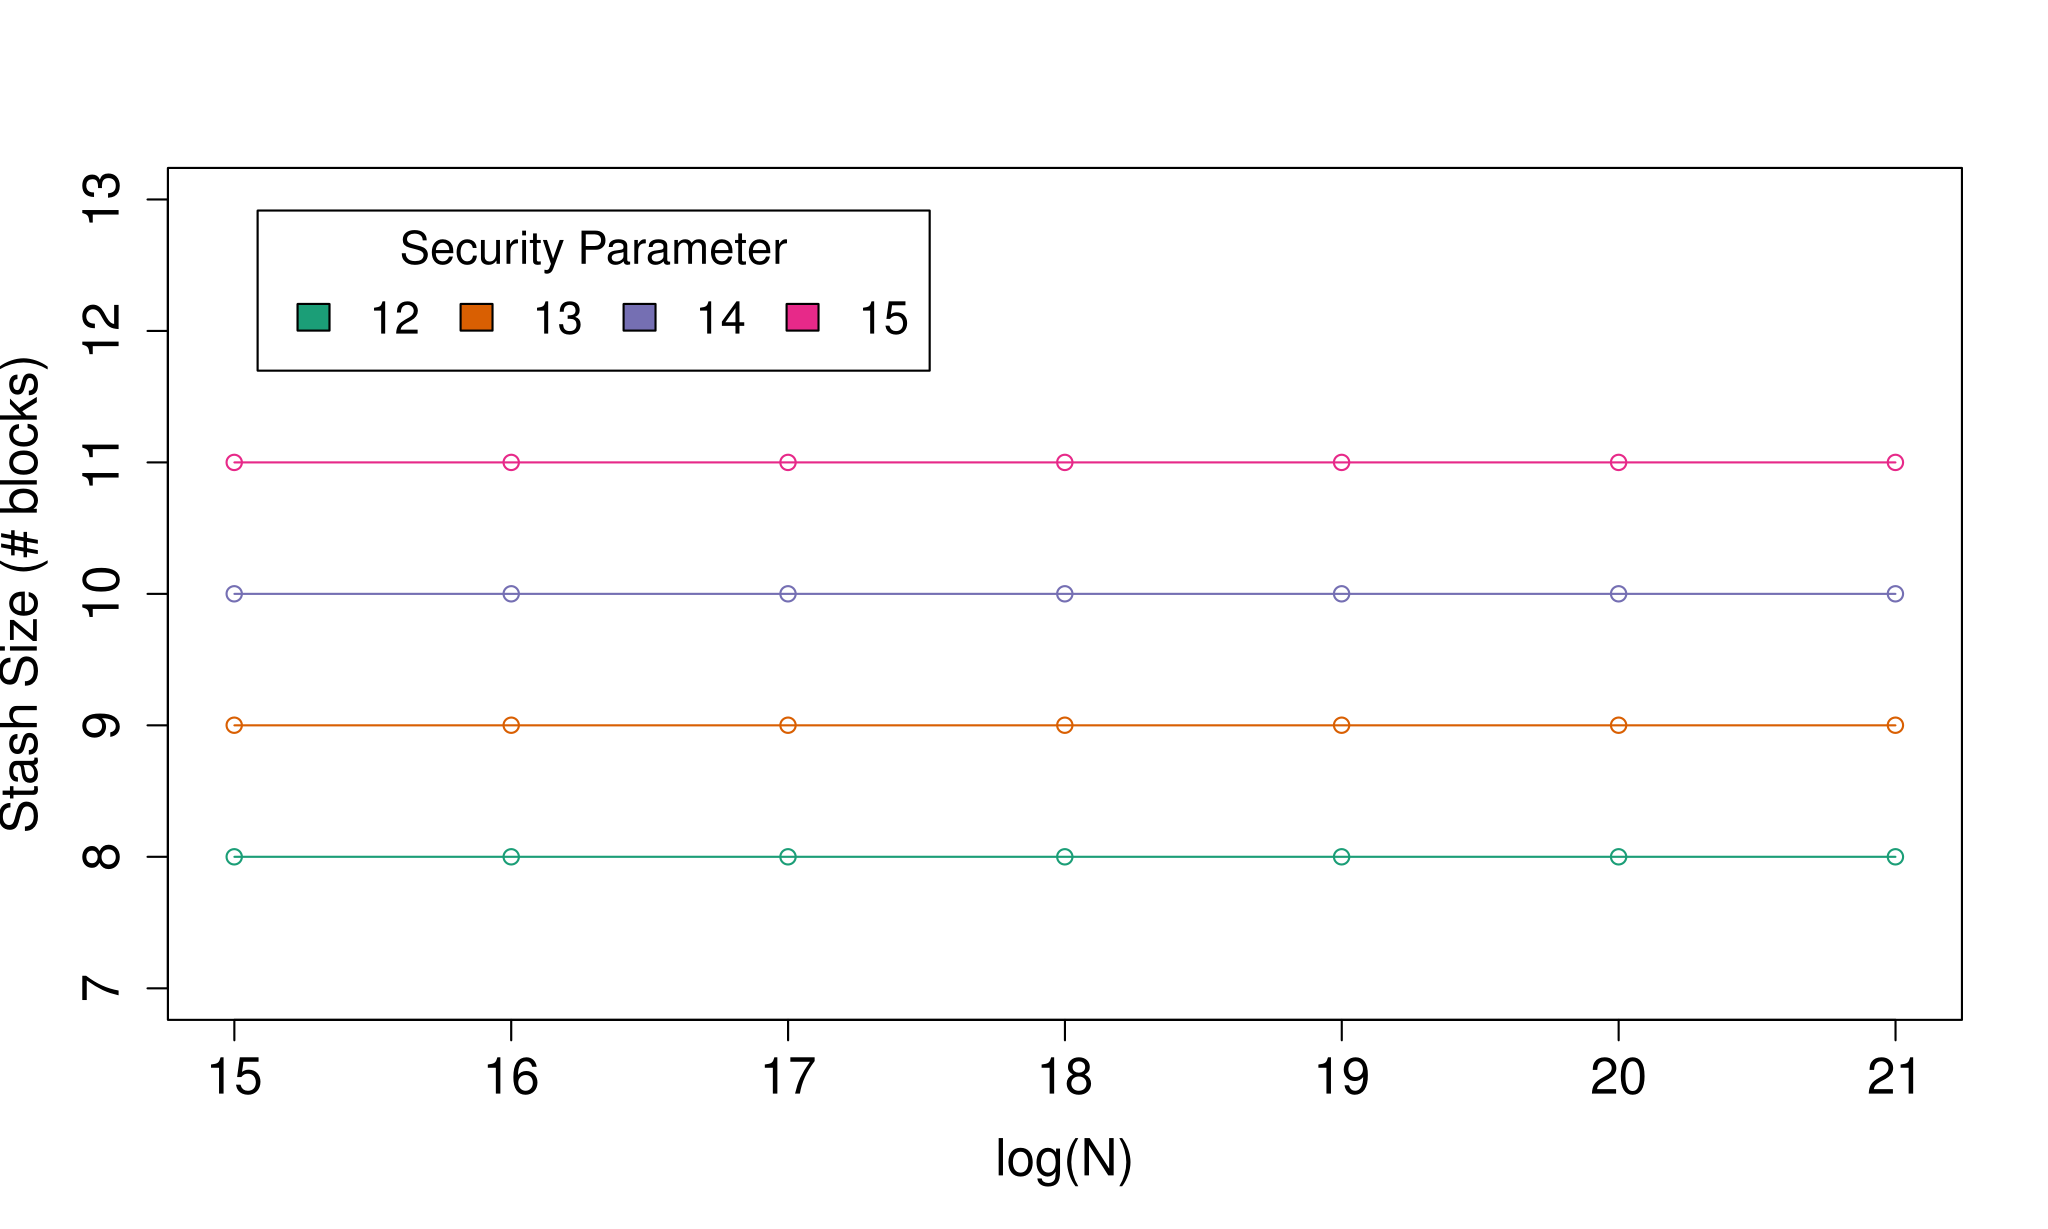
\includegraphics[
				height=5cm,
				keepaspectratio
			]{static/images/stash-size-does-not-depend-on-n.png}

		\end{figure}

	\end{center}

	Figure 4 from~\cite{DBLP:journals/corr/abs-1202-5150}.

\end{frame}
